
% In this chapter, we review the literature on techniques for building compact neural networks.
% First of all, we present, in detail, related work which uses tools from linear algebra and structured matrices. 
% Finally, we present in a more concise way concurrent techniques like using specific memory representation or using neural architecture search.
% These techniques are mostly orthogonal to our contributions.


% We have seen in the Introduction (\Cref{chapter:ch2-introduction}) and Background (\Cref{chapter:ch2-background}) that neural networks tend to be over-parametrized which lead to difficult and expensive training and overfitting.


% In this section, we review the literature for building compact neural networks.
% As seen in the Introduction (\Cref{chapter:ch1-introduction}) and Background (\Cref{chapter:ch2-background}), scaling up networks can lead to an increase in accuracy.
% Researchers have demonstrated that increasing the width of shallow neural networks increased their performance~\cite{howard2017mobilenets,sandler2018mobilenetv2,tan2019mnasnet,zagoruyko2016wide} due to their capacity to capture more fine-grained features.
% Increasing depth is a common and effective way to scale neural networks and many deep architectures have been proposed~\cite{he2016deep, huang2016deep, szegedy2016rethinking,szegedy2017inception,xiao2018dynamical}. 
% The intuition is that deep neural network can capture richer and more complex features.


% Increasing the width of shallow neural networks can increase their performance~\cite{howard2017mobilenets,sandler2018mobilenetv2,tan2019mnasnet,zagoruyko2016wide} due to their capacity to capture more fine-grained features.
% As well, increasing depth is a common and effective approach to capture richer and more complex features and increase performance, many deep architectures have been proposed~\cite{he2016deep,huang2016deep, szegedy2016rethinking,szegedy2017inception,xiao2018dynamical}.
% However, large neural networks lead to difficult and expensive training and overfitting and after observing that a lot of parameters in large neural networks were redundant~\cite{dai2018compressing,frankle2018lottery}, an important question arises: \emph{do neural networks needs to be over-parameterized? And if not, how to build accurate and compact neural networks?} 

%%%%%%%%%%%%%%%%%%%%%%%%%%%%%%%%%%%%%%%%%%%%%%%%%%%%%%%%%%%%%%%%%%%%%%%%%%%%%%%%
\subsection{General Techniques to Build Compact Neural Networks}
%%%%%%%%%%%%%%%%%%%%%%%%%%%%%%%%%%%%%%%%%%%%%%%%%%%%%%%%%%%%%%%%%%%%%%%%%%%%%%%%

As seen in the Introduction (\Cref{chapter:ch1-introduction}), scaling up networks can lead to better accuracy~\cite{tan2019efficientnet,brown2020language}.
However, large neural networks lead to difficult and expensive training and after observing that a lot of parameters in large neural networks were redundant~\cite{dai2018compressing,frankle2018lottery}, an important question arises: \emph{do neural networks need to be over-parameterized? And if not, how to build accurate and compact neural networks?} 

Numerous other directions have been investigated to build compact and cost-effective neural networks without impacting the accuracy.
For example \citet{gupta2015deep,micikevicius2018mixed} have proposed to represent weights with limited numerical precision to reduce training time and memory requirements.
They used half-precision floating-point format instead of single-precision floating-point format which uses 32 bits of computer memory.
In the same direction, \citet{courbariaux2015binaryconnect} have proposed a method to train neural networks with binary weights without an important loss in the accuracy.

An important idea in model compression, proposed by~\citet{bucilua2006model}, is based on the observation that the model used for training is not required to be the same as the one used for inference.
Indeed, compressed models after training can be deployed on smartphones or IoT devices.
Based on this idea, multiple post-processing techniques have been developed: a quantization procedure which consists in converting the weights into a binary or integer formats \emph{after} the training phase~\cite{mellempudi2017ternary,rastegariECCV16}, pruning techniques~\cite{dai2018compressing,han2015deep,lin2017runtime} or sparsity regularizers~\cite{collins2014memory,dai2018compressing,liu2015sparse} which consists in removing redundant weights after training and taking advantage of the sparse structure of the weight matrices.

Sparse neural networks have also been extensively studied since the seminal work of \citet{frankle2018lottery} in which they propose the \emph{Lottery Ticket Hypothesis}. 
This hypothesis states that there exists a sparse subnetwork of a dense neural network that when trained in isolation can match the test accuracy of the original dense network after training for at most the same number of iterations. 
This hypothesis led to a series of works on sparse neural networks \cite{zhou2019deconstructing,malach2019proving,evci2020rigging}.

Moreover, \citet{ba2014deep} have empirically demonstrated that shallow neural networks can learn the complex functions previously learned by other deep neural networks.
This result led \citet{hinton2015distilling} to propose a technique called \emph{model distillation} which consists in training a large complex model using all the available data and resources to be as accurate as possible, then a smaller and more compact model is trained to approximate the first model.
Although interesting for deployment purposes, this approach still requires to train one large network and one shallow, which entails a significant training cost.

\begin{figure}[t]
  \centering
  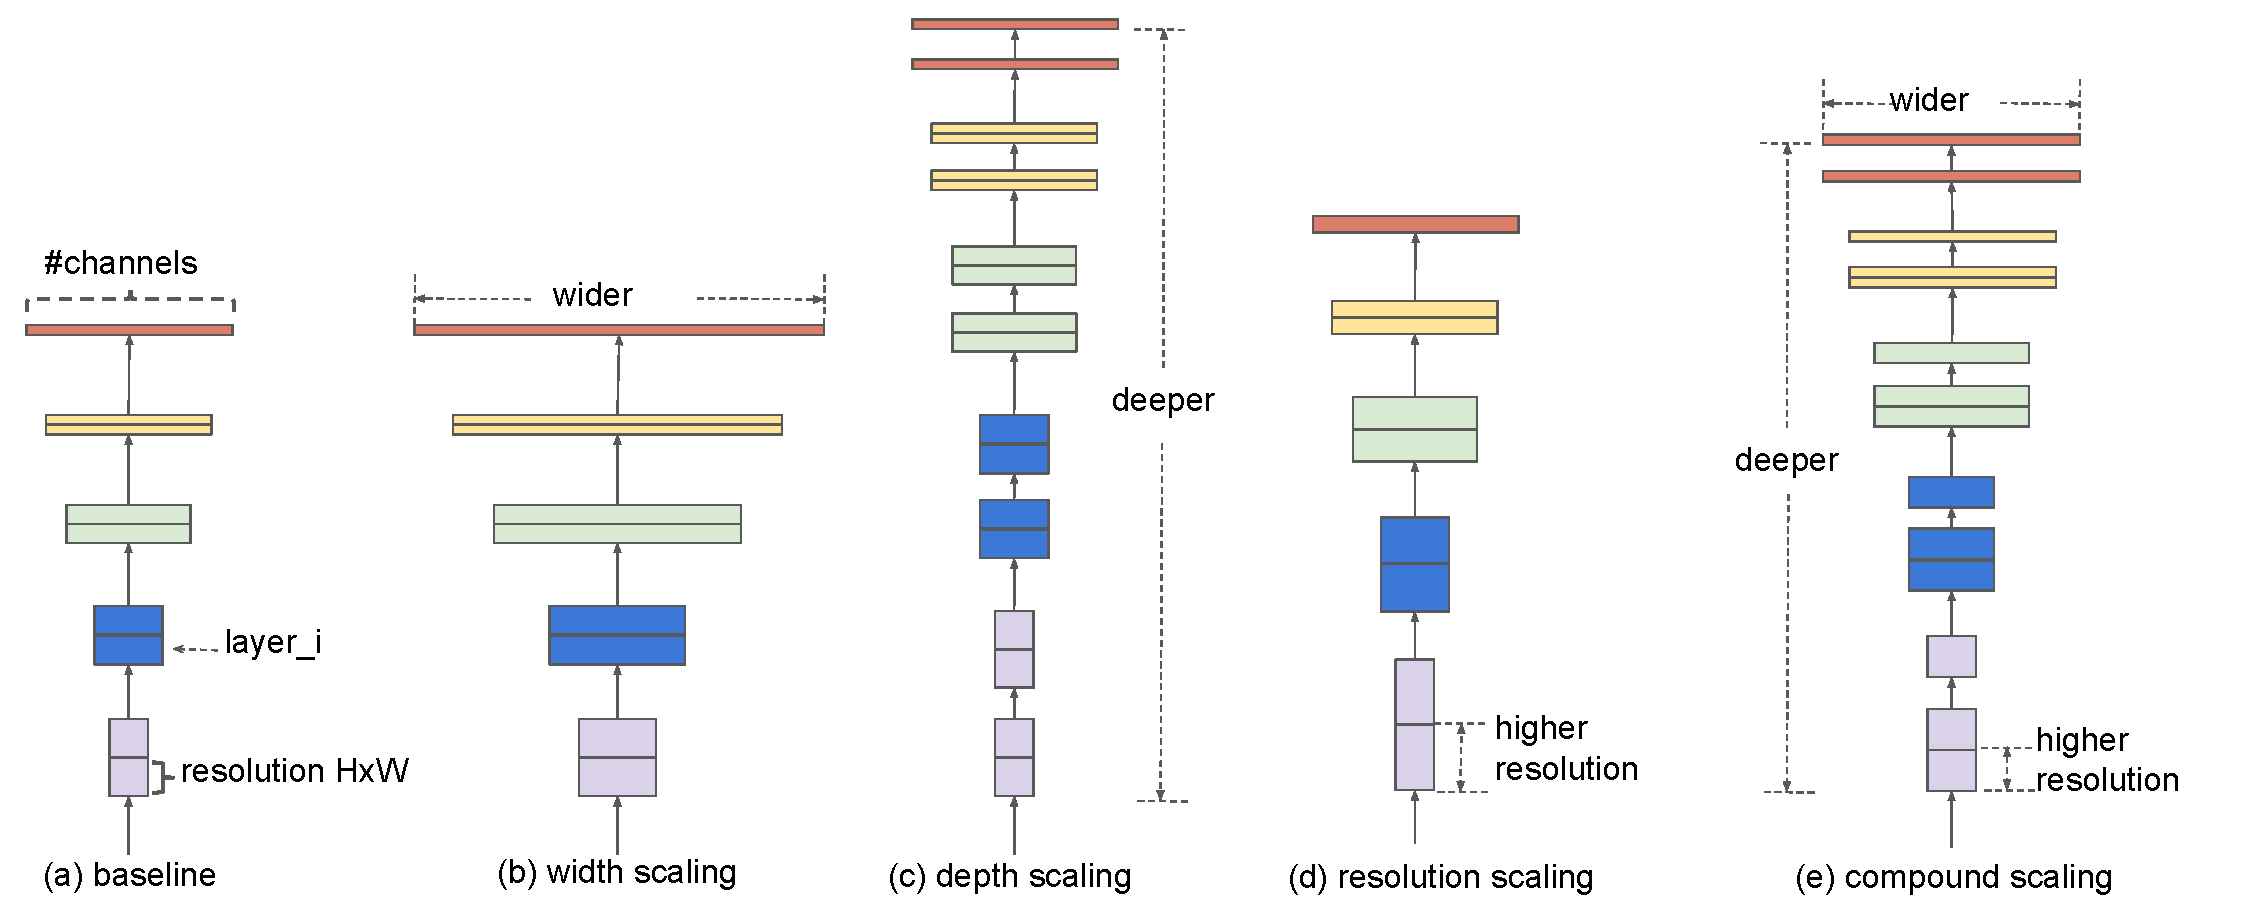
\includegraphics[width=0.80\textwidth]{figures/main/ch3-related_work/scalecompare.pdf}
  \caption{Illustration of the scaling of the EfficientNet architecture.}
  \label{figure:p1-ch3-illustration_efficientnet}
\end{figure}

More recently, \citet{zoph2018learning,real2019regularized} have designed algorithms that automatically tune the width and depth of neural network architectures to obtain the best trade-off between compactness and accuracy.
With this approach, \citet{tan2019efficientnet} found a new compound scaling method that uniformly scales network width and depth leading to efficient and compact architecture.
\Cref{figure:p1-ch3-illustration_efficientnet} illustrates the different scaling proposed by~\citet{tan2019efficientnet}.

% Finally, in the context of deep learning, compact representations have gained much attention over the past years as a way to compress models or to reduce memory requirements.
% In this thesis, we focus on building compact neural networks with structured matrices.
% Hereafter, we present a comprehensive overview of the existing techniques in this line of research.



% --> Compact Neural Networks Architecture

% Without consideration of specific memory representations, data structures or structured linear layers, it is still possible to design compact neural networks.
%
% However, researchers have demonstrated that increasing the width of shallow neural networks increased their performance~\cite{howard2017mobilenets,sandler2018mobilenetv2,tan2019mnasnet,zagoruyko2016wide} due to their capacity to capture more fine-grained features.
% Finally, depth is a common and effective way to scale neural networks and many deep architectures have been proposed~\cite{he2016deep, huang2016deep, szegedy2016rethinking,szegedy2017inception,xiao2018dynamical}. 
% The intuition is that deep neural network can capture richer and more complex features.
%
% After observing that large and deep neural networks outperformed shallow ones \cite{huang2019gpipe,brown2020language} and the observation that a lot of parameters in large neural networks were redundant~\cite{dai2018compressing,frankle2018lottery}, an important question arises: \emph{do neural networks needs to be large \ie, deep and wide, and if not, which architecture provides the best accuracy?} 

% \citet{ba2014deep} tried to answer this question and empirically demonstrated that shallow neural networks can learn the complex functions previously learned by another neural network. 
% This observation was then leveraged by~\citet{hinton2015distilling} for compressing trained neural networks.
% Their technique, called \emph{model distillation}, consists to train a large complex model using all the available data and resources to be as accurate as possible, then a smaller and more compact model is trained to approximate the first model.
% Although, this approach can be interesting for deployment purposes, it is still required to train one large network and one shallow, which entails a significant training cost.
%
% Instead of compressing the model after the training step, researchers still tried to design architectures that are compact by nature but finding the best trade-off between depth, width and performance has proved to be a tedious work.
% In order to scale the search, recent works have devised algorithms to automatically find the best architecture for a specific use case.
% \citet{zoph2018learning,real2019regularized} have tried to tune the wide and depth of neural network architectures to obtain the best trade-off between efficiency and accuracy but these methods required a lot of manual tuning.
% More recently, with a similar method, \citet{tan2019efficientnet} found a new compound scaling method to uniformly scales network width, depth, and resolution leading to groundbreaking result in terms of efficiency and accuracy.




%%%%%%%%%%%%%%%%%%%%%%%%%%%%%%%%%%%%%%%%%%%%%%%%%%%%%%%%%%%%%%%%%%%%%%%%%%%%%%%%
\subsection{Building Compact Neural Networks with Structured Matrices}
\label{subsection:ch3-building_compact_neural_networks_with_structured_matrices}
%%%%%%%%%%%%%%%%%%%%%%%%%%%%%%%%%%%%%%%%%%%%%%%%%%%%%%%%%%%%%%%%%%%%%%%%%%%%%%%%

% An effective method to build compact neural networks is to constrain the hypothesis space in which the learning algorithm ``chooses'' the predictor.
% As seen in \Cref{chapter:ch2-background}, this constraint is called \emph{inductive bias}. 

% Another way of constraining the weight representation and reduce the memory requirement of neural networks is to impose a \emph{structure} on weight matrices. 

% The idea of building compact neural networks with structured matrices consists of replacing the weight matrices $\Wmat^{(i)}$ with \emph{structured matrices}.


% A structured matrix is a $n \times n$ matrix whose entries have a formulaic relationship, allowing the matrix to be represented with fewer than $n^2$ parameters.
% The formulaic relationship between entries is an important feature to consider, for example, a sparse matrix has fewer than $n^2$ parameters but does not have a clear relationship between its entries.

% by using \emph{structured neural networks}. 
% The idea of structured neural networks consists of replacing the dense weight matrices with \emph{structured} ones.

An effective method to build compact neural networks is to constrain the hypothesis space by imposing a \emph{structure} on the weight matrices which constitute the different layers of the network.
% A structured matrix is a $n \times n$ matrix which can be represented with fewer than $n^2$ parameters and where the entries are distributed along specific rules.

%%%%%%%%%%%%%%%%%%%%%%%%%%%%%%%%%%%%%%%%%%%%%%%%%%%%%%%%%%%%%%%%%%%%%%%%%%%%%%%%
\paragraph{Structured Neural Networks with Low Rank Approximation} ~\\
%%%%%%%%%%%%%%%%%%%%%%%%%%%%%%%%%%%%%%%%%%%%%%%%%%%%%%%%%%%%%%%%%%%%%%%%%%%%%%%%

\noindent
For example, \citet{sainath2013lowrank} were among the first to use low-rank matrices in deep learning contexts followed by the work of~\citet{jaderberg2014speeding,yu2017compressing}.
Their work consists in replacing the weight matrices of size $n \times m$ by the product of two rectangular matrices of size $n \times r$ and $r \times m$, where $r$ corresponds to the rank of the new matrix. 
In order to reduce the number of parameters, the rank $r$ is chosen to be small such that $r \ll \min(m, n)$.
By representing the weight matrices with a low-rank decomposition, one can reduce the storage from $mn$ parameters to $(mr + nr)$ and accelerate the matrix-vector product from $\bigO(mn)$ to $\bigO(mr + rn)$.
To enforce the low-rank constraint, reduced storage and computation time during training, the authors trained the coefficients of the two rectangular matrices directly. 
Formally, let $\Wmat \in \Rbb^{n \times m}$ be a weight matrix and let $\widetilde{\Wmat}$ be the low-rank approximation of rank $r$ of the matrix $\Wmat$.
Then, the low-matrix $\widetilde{\Wmat}$ can be decomposed by the product of two rectangular matrices $\Umat \in \Rbb^{n \times r}$ and $\Vmat \in \Rbb^{r \times m}$ such that $\widetilde{\Wmat} = \Umat \Vmat$.
Therefore, a neural network layer with low-rank approximation can be expressed as follows:
\begin{equation}
  \layer_{\Umat, \Vmat, \bvec} (\xvec) = \act\left( \Umat \Vmat \xvec + \bvec \right) .
\end{equation}
The scalar $r$ defining the size of the two rectangular matrices becomes an hyper-parameter and controls the trade-off between the expressivity and compactness of the layer. 

In the same vein, \citet{oseledets2011tensor} have proposed the \emph{Tensor Train decomposition} (TT-decomposition), which is based on the tensor rank decomposition (Tucker decomposition) proposed by~\citet{hitchcock1927expression} and named after \citet{tucker1966some}.
The TT-decomposition is defined as follows.
Let $\boldsymbol{\Aset} \in \Rbb^{n_1 \times n_2 \times \dots \times n_{d-1} \times n_d}$ be a $d$-dimensional tensor.
The Tensor-Train Decomposition factorizes $\boldsymbol{\Aset}$ in a product of third-order tensors and it is given by: 
\begin{equation}
  (\boldsymbol{\Aset})_{(i_1,\dots,i_d)} = (\Gmat^{(1)})_{(i_1, :)} (\boldsymbol{\Gset}^{(2)})_{(:, i_2, :)} (\boldsymbol{\Gset}^{(3)})_{(:, i_3, :)} \dots (\Gmat^{(d)})_{(:, i_d)}
\end{equation}
where $\Gmat^{(i)}$ are matrices and $\boldsymbol{\Gset}^{(i)}$ are third-order tensors of size $r_{i} \times r_{i+1}$ called \emph{TT-cores}.
The sequence $\{r_k\}_{k=0}^d$ is referred to as the ranks of the TT-representation.
The above equation can be equivalently rewritten as a sum of elements of the TT-cores:
\begin{equation}
  (\boldsymbol{\Aset})_{(i_1,\dots,i_d)} = \sum_{\alpha_1, \dots, \alpha_{d-1}} (\Gmat^{(1)})_{(i_1, \alpha_1)} (\boldsymbol{\Gset}^{(2)})_{(\alpha_1, i_2, \alpha_2)} \dots (\Gmat^{(d)})_{(\alpha_{d-1}, i_d)}
\end{equation}
\citet{oseledets2011tensor} have shown that for an arbitrary tensor $\boldsymbol{\Aset}$, several TT-representations exist with different ranks.
The TT-decomposition can be very efficient in terms of memory requirement if the ranks are small.
Indeed, the tensor $\boldsymbol{\Aset}$ has $\prod_{k=1}^{d} n_k$ values compared with $\sum_{k=1}^d n_k r_{k-1} r_k$ values.

The TT-decomposition has been extensively used in the context of deep learning.
\citet{novikov2015tensorizing} was one of the first to use this technique to reduce the number of parameters of neural networks by using the decomposition to replace the fully connected layer of the VGG architecture~\cite{simonyan2014very}.
They reported a compression factor of the dense weight matrix up to 200000 times leading to the compression factor of the whole network up to 7 times with only 0.3 point drop of TOP-5 accuracy on ImageNet~\cite{deng2009imagenet}.
With this work, \citet{novikov2015tensorizing} have demonstrated that the TT-decomposition allows an important reduction of the number of parameters while preserving the expressive power of the layers.
Later, the TT-decomposition was used in other types of architectures.
\citet{garipov16ttconv} used it to compress convolution layers as well as fully connected layers.
\citet{yang2017tensor} used it in the context of video classification, \citet{tjandra2017compressing} compressed the layers of recurrent neural networks and finally, \citet{xindian2019tensorized} developed a compact architecture based on TT-decomposition for Language Modeling.

However, the Tensor-Train decomposition has some limitations.
Although it can reduce the number of parameters when the ranks are low, finding the best alignment of the tensor dimensions in order to find the best optimized TT-cores remains a challenging problem, as stated by~\citet{pan2019compressing}.


% In the same vein, \citet{novikov2015tensorizing} have proposed a generalization of low-rank decomposition.
% Instead of searching for low-rank approximation of the weight matrices, they consider multi-dimensional tensors and apply the \emph{Tensor Train decomposition} algorithm \cite{oseledets2011tensor}.
% The Tensor Train decomposition allows an important reduction of the number of parameters while preserving the expressive power of the layers.



%%%%%%%%%%%%%%%%%%%%%%%%%%%%%%%%%%%%%%%%%%%%%%%%%%%%%%%%%%%%%%%%%%%%%%%%%%%%%%%%
\paragraph{Neural Networks with Diagonal and Circulant Matrices} ~\\
%%%%%%%%%%%%%%%%%%%%%%%%%%%%%%%%%%%%%%%%%%%%%%%%%%%%%%%%%%%%%%%%%%%%%%%%%%%%%%%%

\noindent

% Since the seminal work of \citet{ailon2009fast}, structured transforms have been extensively studied in the context of dimensionality reduction and random projections.
% For example, the Fastfood transform which was proposed by \cite{le2013fastfood}  
%
% Other types of structured transforms have been used to  


% The authors have replaced dense matrices of fully connected layers with adaptive structured matrices of the form: $\Smat\Hmat\Gmat\mathbf{\Pi}\Hmat\Bmat$ where $\Smat$, $\Gmat$, and $\Bmat$ are adaptive diagonal matrices, $\mathbf{\Pi}$ is a random permutation matrix, and $\Hmat$ is the Walsh-Hadamard matrix.


% Other types of decomposition have been used to reduce the number of parameters of neural networks.
% The Fastfood transform which was originally used for approximating kernel expansions~\cite{le2013fastfood}, was later used in neural networks by~\citet{yang2015deep} leading to the Deep Fried Convnets architecture.
% The authors have replaced dense matrices of fully connected layers with adaptive structured matrices of the form: $\Smat\Hmat\Gmat\mathbf{\Pi}\Hmat\Bmat$ where $\Smat$, $\Gmat$, and $\Bmat$ are adaptive diagonal matrices, $\mathbf{\Pi}$ is a random permutation matrix, and $\Hmat$ is the Walsh-Hadamard matrix.
% Later, the \emph{Structured Spinners} transform of the form: $\Hmat\Dmat^{(3)} \Hmat\Dmat^{(2)} \Hmat\Dmat^{(1)}$, where $\Hmat$ is the Walsh-Hadamard matrix, and $\Dmat^{(i)}$ for $i \in {1, 2, 3}$ is a random $\pm1$-diagonal matrix, was originally proposed by~\citet{andoni2015practical} and used in deep learning settings by~\citet{bojarski2017structured}.



% Key to Fastfood is the observation that Hadamard 
% matrices when combined with diagonal Gaussian
% matrices exhibit properties similar to dense
% Gaussian random matrices. Yet unlike the
% latter, Hadamard and diagonal matrices are
% inexpensive to multiply and store.

% which can be viewed as a generalized class of Fourier transforms.

% Decomposition with structured matrices of interest for the contributions of this thesis are the ones based on diagonal and circulant matrices.

% More practically, \citet{hinrichs2011johnson} have shown that the \DC transform $\xvec \mapsto \Dmat \Cmat \xvec$, where the matrix $\Dmat$ is a diagonal matrix with entries sampled from $\{1, -1\}$ and $\Cmat$ is a circulant matrix based on a sequence of independent identically distributed random variables respect the \citeauthor{johnson1984extensions} lemma.
\citet{cheng2015exploration} proposed to replace the weight matrix of a fully connected layer by the product of a circulant and a diagonal matrix leading to following structured layer:
\begin{equation}
  \layer_{\Dmat, \Cmat, \bvec} (\xvec) = \act \left( \Dmat \Cmat \xvec + \bvec \right) \enspace,
\end{equation}
where the circulant matrix is learned by a gradient-based optimization algorithm and the diagonal matrix entries are sampled at random in $\{-1, 1\}$. 
The idea of replacing dense matrices with circulant ones comes from their use in dimensionality reduction with the \emph{fast Johnson-Lindenstrauss transform}~\cite{hinrichs2011johnson,vybiral2011variant}, binary embedding~\cite{yu2014circulant}, and kernel approximation~\cite{yu2015compact}, etc.
Circulant matrices exhibit several interesting properties from the perspective of numerical computations.
Recall from \Cref{theorem:ch2-diagonalization_circulant_matrix} that circulant matrices can be diagonalized with the Fourier Transform as follows:
\begin{equation}
  \Cmat = \frac{1}{n} \Umat_n^* \diag(\Umat_n \cvec) \Umat_n \enspace.
\end{equation}
where the vector $\cvec$ corresponds to the first columns of the matrix $\Cmat$.
This decomposition allows a compact representation in memory ($n$ values instead of $n^2$) and efficient matrix-vector product with the FFT algorithm (see \Cref{algorithm:ch2-matrix_vector_product_circulant_matrix}).
% Thanks to this decomposition, circulant matrices exhibit several interesting properties from the perspective of numerical computations. Most importantly, any $n \times n$ circulant matrix $\Cmat$ can be represented using only $n$ coefficients instead of the $n^2$ coefficients required to represent classical unstructured. In addition, the matrix-vector product is simplified from O(n 2) to O(n log(n)) using the convolution theorem.
% Thanks to this decomposition, circulant matrices offer a compact representation in memory (they can be expressed with only $n$ values instead of $n^2$) and an efficient matrix-vector product with the FFT algorithm (see \Cref{algorithm:ch2-matrix_vector_product_circulant_matrix}).
Despite the reduction of expressivity, \citet{cheng2015exploration} demonstrated good empirical results using only a fraction of the original weights (90\% reduction). 


\citet{moczulski2016acdc} built upon the work of~\citet{cheng2015exploration} and \citet{huhtanen2015factoring} and introduced two \emph{Structured Efficient Linear Layers} (SELL) based on the Fourier and cosine transforms.
First, by observing that the DC transform cannot express an arbitrary linear operator they proposed to apply the result of \citet{huhtanen2015factoring} which states that almost all matrices can be decomposed as a product of DC transforms.
\begin{theorem}[Reformulation from \citet{huhtanen2015factoring}] \label{theorem:ch3-huhtanen}
  For every matrix $\Mmat \in \Cbb^{n \times n}$, for any $\epsilon > 0$, there exists a sequence of matrices $\{ \Amat^{(i)} \}_{i \in [2n-1]}$ where $\Amat^{(i)}$ is a circulant matrix if $i$ is odd, and a diagonal matrix otherwise, such that $\norm{\Amat^{(1)} \ldots \Amat^{(2n-1)} - \Mmat} < \epsilon$.
\end{theorem}
\noindent
Based on this result, they proposed to parameterize the layers of a neural network with $k$ products of diagonal and circulant matrices as follows:
\begin{equation} \label{equation:acdc_layer}
  \layer_{\Dmat, \Cmat, \bvec} (\xvec) = \act \left( \left(\prod_{i = 1}^{k} \Dmat^{(i)} \Cmat^{(i)} \right) \xvec + \bvec \right)
\end{equation}
where $\Dmat$ and $\Cmat$ are sequences of $k$ diagonal and circulant matrices respectively.
This structured layer is therefore parameterized by $n(2k+1)$ values and the value $k$ becomes a hyper-parameter controlling the trade-off between compactness and expressivity. 
By diagonalizing the circulant matrix, the layer in \Cref{equation:acdc_layer} can be expressed as a product of diagonal matrices and the Fourier transform as follows:
\begin{equation} \label{equation:ch3-laye_acdc}
  \layer^\act_{\dvec, \cvec, \bvec} (\xvec) = \act \left(\frac{1}{n^k} \left(\prod_{i = 1}^{k} \diag\left(\dvec^{(i)}\right) \Umat_n^* \diag\left(\Umat_n \cvec^{(i)}\right) \Umat_n \right) \xvec + \bvec \right)
\end{equation}
\noindent
Although interesting and demonstrating good empirical results, the work of~\citet{moczulski2016acdc} suffers from multiple limitations. 
First, the result from~\citet{huhtanen2015factoring} is expressed with respect to $n$, the size of the matrices $\Amat$.
Therefore, the theorem does not provide any insights regarding the expressive power of $k$ factors when $k$ is much lower than $2n-1$ as it is the case in most practical scenarios they consider.
Finally, in order to stay in the real domain, they replaced the Fourier transform in~\Cref{equation:ch3-laye_acdc} with the cosine transform thus learning a different kind of linear transform (see the work of~\citet{sanchez1995diagonalizing} which characterizes the matrices diagonalizable by the cosine transform).
Furthermore, because the cosine transform does not diagonalize circulant matrices, \Cref{theorem:ch3-huhtanen} no longer applies.


% \vspace{0.3cm}

%%%%%%%%%%%%%%%%%%%%%%%%%%%%%%%%%%%%%%%%%%%%%%%%%%%%%%%%%%%%%%%%%%%%%%%%%%%%%%%%
\paragraph{General Representation of Structured Linear Maps: LDR and K-Matrices} ~\\
%%%%%%%%%%%%%%%%%%%%%%%%%%%%%%%%%%%%%%%%%%%%%%%%%%%%%%%%%%%%%%%%%%%%%%%%%%%%%%%%

\vspace{-0.5cm}

General framework for structured matrices that reduce the memory footprint but also accelerate matrix-vector product operations have been used to build compact neural networks.
\citet{sindhwani2015structured} have used the notion of low displacement rank presented in \Cref{subsection:ch2-general_frameworks_for_structured_matrices} to learn a broad family of structured matrices.
Recall from~\Cref{theorem:ch2-toeplitz_like} that all matrices expressed as the following sum of products are called \emph{Toeplitz-like} matrices:
\begin{equation}
    \Mmat = \sum_{j=1}^{r} \Zmat_1(\gvec^{(j)}) \Zmat_{-1}(\Jmat_n \hvec^{(j)})
\end{equation}
where $\Zmat_f$ is an $f$-circulant matrix defined in \Cref{definition:ch2-f_circulant_matrix} and $\Gmat = \leftmat \gvec^{(1)} \ldots \gvec^{(r)} \rightmat, \Hmat = \leftmat \hvec^{(1)} \ldots \hvec^{(r)} \rightmat \in \Rbb^{n \times r}$ with $r \ll n$.
More precisely, \citet{sindhwani2015structured} proposed to learn Toeplitz-like matrices by learning the factors $\Gmat$ and $\Hmat$. 
Therefore, they proposed the following parameterized layer:
\begin{equation}
  \layer_{\Gmat, \Hmat, \bvec}(\xvec) = \act \left( \left(\sum_{j=1}^{r} \Zmat_1\left(\gvec^{(j)}\right) \Zmat_{-1}\left(\Jmat_n \hvec^{(j)}\right) \right) \xvec + \bvec \right)
\end{equation}
where the rank $r$ is a hyper-parameter and controls the number of parameters of the layer.
In addition to offer fast matrix-vector product, they have showed that this class of layers is very rich from a modeling perspective.
More precisely, they characterize the expressivity of the layer as follows: 
\begin{theorem}[LDR expressivity \citet{pan2001structured,sindhwani2015structured}] ~\\
  The set of all $n \times n$ matrices that can be written as, $\sum_{i=1}^{r} \Zmat_1(\gvec^{(i)}) \Zmat_{-1}(\hvec^{(i)})$
  for some $\Gmat = \leftmat \gvec^{(1)} \ldots \gvec^{(r)} \rightmat,
  \Hmat = \leftmat \hvec^{(1)} \ldots \hvec^{(r)} \rightmat \in \Rbb^{n \times r}$ contains:
  \begin{compactitem}
    \item All $n \times n$ Circulant and Skew-Circulant matrices for $r \geq 1$.
    \item All $n \times n$ Toeplitz matrices for $r \geq 2$.
    \item Inverses of Toeplitz matrices for $r \geq 2$.
    \item All products of the form $\Amat^{(1)} \ldots \Amat^{(t)}$ for any $t \leq \frac{r}{2}$.
    \item All linear combinations of the form $\sum_{i=1}^p \beta_i \Amat^{(1, i)} \ldots \Amat^{(t, i)}$ for any $t \leq \frac{r}{2p}$.
    \item All $n\times n$ matrices for $r=n$.
  \end{compactitem}
  where each $\Amat^{(i)}$ above is a Toeplitz matrix or the inverse of a Toeplitz matrix. 
\end{theorem}
\noindent

In the same line of work, \citet{thomas2018learning} have proposed neural network layers directly form the Krylov decomposition presented in~\Cref{theorem:ch2-krylov_decomposition} which encompasses an even larger family of structured matrices including Toeplitz-like, Vandermonde-like, Cauchy-like ones.
Despite being elegant and general, we found that the LDR framework suffers from several limits which are inherent to its generality and makes it difficult to use in the context of deep neural networks.
% First, the training procedure for learning LDR matrices is highly involved and implies many complex mathematical objects such as Krylov matrices.
As acknowledged by the authors, the number of parameters required to represent a given structured matrix (a Toeplitz matrix) in practice is unnecessarily high (higher than required in theory) making the training very hard. 



More recently, another type of generalization of structured linear maps has been proposed by~\citet{dao2019learning,dao2020kaleidoscope}.
They introduced a family of matrices called \emph{kaleidoscope matrices} (K-matrices) which are the product of sparse matrices with specific predefined sparsity patterns.
They showed that this type of matrices can capture any sparse matrix with near-optimal space (parameter) and time (arithmetic operation) complexity.
The authors claim that their structured linear maps can capture more common structures with a few numbers of parameters than the displacement operators presented above.
More precisely, their representation is based on products of a particular building block known as a butterfly matrix introduced by~\citet{parker1995random}.
Butterfly matrices have been extensively used in numerical linear algebra~\cite{parker1995random,li2015butterfly} and machine learning~\cite{mathieu2014fast,jing2017tunable,munkhoeva2018quadrature,dao2019learning,choromanski2019unifying}.





